\usetikzlibrary{trees}


\newcommand{\cara}{\fontsize{10}{6}\selectfont\color{redsol} \ManFace}
\begin{multicols}{2}

\cappar Te gustan los Simpsons? ¿qué opinas de esta conocida serie? ¿Te sorprenderías si te contase que en los episodios de Los Simpsons hay temas matemáticos y además relacionados a matemáticas muy sofisticadas? Pues es así y la razón es que trabajan varios genios matemáticos en la serie. Al Jean, el productor ejecutivo, fue admitido para estudiar ciencias exactas en Harvard cuando tenía 16 años. Jeff Westbrook renunció a un puesto de investigador en Yale para escribir guiones de Los Simpsons. David S. Cohen, otro guionista, llegó al equipo después de resolver uno de los grandes problemas de la geometría. 

Hace poco se publicó el libro \emph{The Simpsons and their Mathematical Secrets} publicado por Simon Sigh, doctor en física teórica y conocido divulgador. En este nos cuenta muchas de  esas referencias matemáticas que aparecen en la serie de Los Simpsons. Puedes seguir sus noticias en la siguiente web \url{http://www.simonsingh.net/Simpsons_Mathematics/}.

Por ejemplo en el capítulo 22 de la sesión 17ª aparece en el videomarcador de un partido que Homer y Marge están viendo algo así:

\begin{mybox}
\huge{TONIGHT'S ATTENDANCE}
\begin{description}
\item[A)] 8128
\item[B)] 8208
\item[C)] 8191
\item[D)] No way to tell
\end{description}
\end{mybox}

No parece nada especial, ¿verdad? Pues lo es, te explicamos a continuación que significado tienen estos números:
\begin{description}
\item[A)] 8128 es un número perfecto: esto es cuando el número es suma de todos sus divisores menor que el. Un ejemplo sencillo es el 28 que es suma de 1,2,4,7 y 14. 
\item[B)] 8208 es una número narcisista ya que si sumamos las cuartas pòtencias de sus cifras nos da el mismo. Esto es, $8^4+2^4+0^4+8^4=8208$.
\item[C)] 8191 es un número primo: sus únicos divisores son 1 y el número mismo.
\end{description}

\section*{El desafío: ¿Cuánto vale mi televisor?}
Un señor acaba de inaugurar un hotel con 72 habitaciones.
Entre los objetos que tuvo que distribuir en cada una de ellas
había un televisor. El gerente que tenía que ocuparse del tema
fue a una empresa de electrodomésticos y compró 72 televisores
iguales.

Cuando hacían la revisión de todas las inversiones, el dueño
le pidió al gerente que le diera el recibo de compra, y allí descubrieron que el papel se había humedecido y había borroneado
algunos números. Con todo, se podía ver que era un número de
cinco cifras, pero se habían borrado la primera y la última. Se
veía algo así:
\begin{center}\huge{X679Y}\end{center}
¿Puedes averiguar por cuánto salió cada televisor sabiendo que pagó por cada uno de ellos un número entero?

\section*{\textcolor{redsol}{Soluciones del número anterior}}
\subsection*{El chisme}
Cuando llegó el caballero extranjero eran las 10 de la mañana y a las 10:15 de la mañana ya 4 personas conocían el chisme, el extranjero y tres más de la ciudad. Un cuarto de hora después cada una de las personas de la ciudad se lo comunicó a tres personas más. Así a las 10 y media eran conocedoras $1+3+(3*3)$ personas. Un cuarto de hora más tarde sería: $1+3+(3*3)+(3*3*3)=1+3^2+3^3$, etc. Es decir, podemos representar el problema como la suma de la sucesión $a_n=3^{n-1}$ donde el contador $n$ representará el tiempo. Para $n=1$, supondremos son las 10 de la mañana y cada aumento de $n$ significará un cuarto de hora. Con este planteamiento nuestro problema se resuelve solucionando la siguiente desigualdad:
\begin{equation}
1+3+3^2+3^3+\dots+3^{n-1}=\sum_{i=1}^n a_n \leq 50.000
\end{equation}

La sucesión $a_n$ es una progresión geométrica, esto es que cada término es generado por el anterior multiplicando simpre por la misma cantidad que se denomina \emph{razón}. La sucesión $a_n$ es una progresión geométrica de razón 3 y dejamos como ejercicio al lector que compruebe el valor de la suma:$\sum_{i=1}^n a_n=\frac{3^{n}-1}{2}$ (debe recurrir a la fórmula de la suma de una progresión geométrica\footnote{Si la fórmula general de un sucesión geométrica es $a_n=a_1 \cdot r^{n-1}$ siendo $a_1$ el primer elemento y $r$ la razón. La suma $S_n$ de los $n$ primeros términos de la sucesión es:
$$
S_n=\frac{a_1 (r^{n-1}-1)}{r-1}.
$$. 
}.

Resolvemos la inecuación como sigue:
$$
\frac{3^{n}-1}{2} \leq 50.000 \,;\, 3^n<100,001  \,;\, n\leq 10.4.
$$

De esta manera para $n=11$ ya toda la ciudad conoce el rumor y $n=11$ nos dan las 12 y media de la mañana. Es decir que un poco antes de las 12 y media de la mañana el rumor ha sido propagado por toda la ciudad, ¡increíble! 

Mostramos a continuación una abstracción de como se propaga un rumor:
\begin{center}
\begin{tikzpicture}
    \node {\cara}
    child[grow=195] {node  {\cara} 
         child[grow=195, level distance=1cm] {node  {\cara}}
    child[grow=270,level distance=1cm] {node  {\cara}}
    child[grow=345,level distance=1cm] {node  {\cara}}}
    child[grow=270] {node  {\cara} child[grow=195, level distance=1cm] {node  {\cara}}
    child[grow=270,level distance=1cm] {node  {\cara}}
    child[grow=345,level distance=1cm] {node  {\cara}}}
    child[grow=345] {node  {\cara} child[grow=195, level distance=1cm] {node  {\cara}}
    child[grow=270,level distance=1cm] {node  {\cara}}
    child[grow=345,level distance=1cm] {node  {\cara}}};
    
    %child[grow=180, level distance=3cm]{node {\cara}}
    %child[grow=270, level distance=2cm] {node {\cara}}}
    %;
\end{tikzpicture}
\end{center}

\subsection*{Belleza al ganar}
La otra solución que se propone de la jugada que propusimos en el número anterior y que mostramos a continuación
\begin{figure}[!ht]
\centering 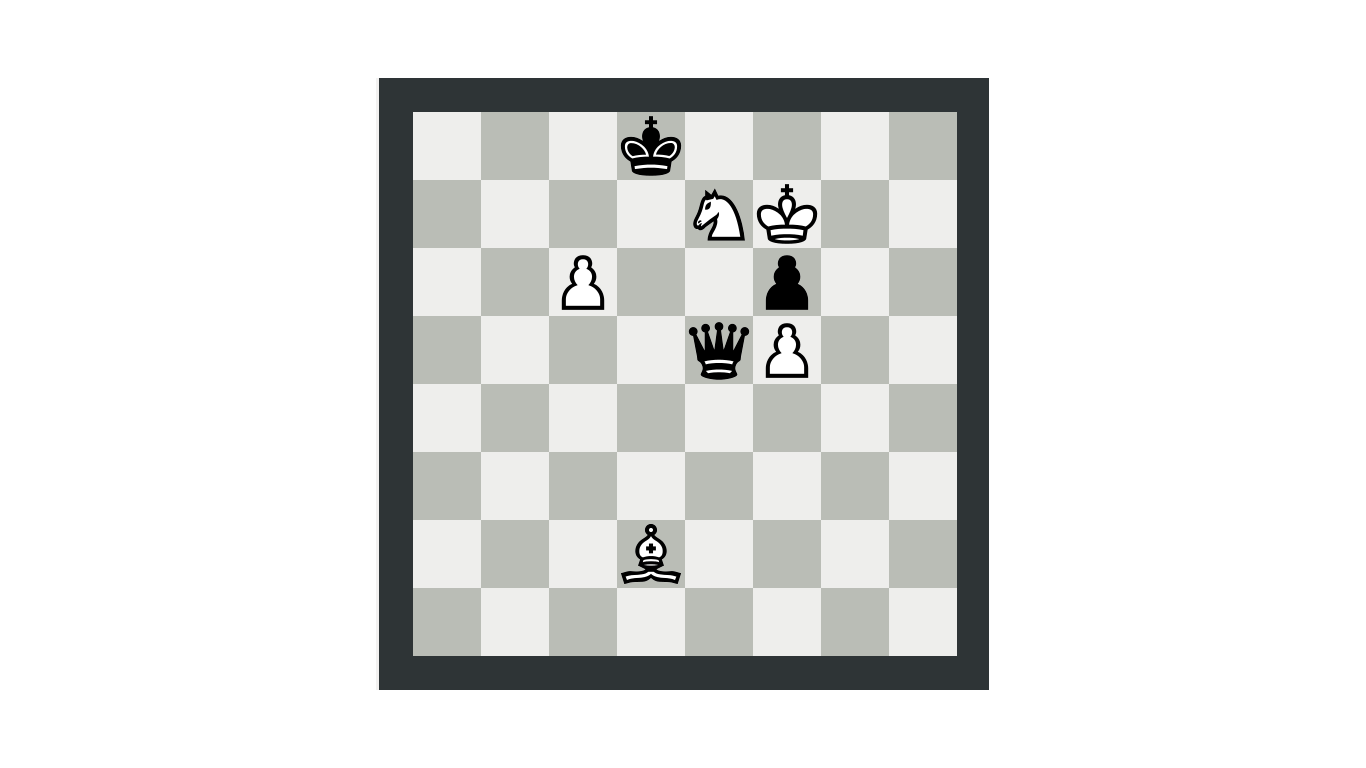
\includegraphics[scale=0.2]{partida2.png}
\caption{Reto ajedrecístico}\label{partida}
\end{figure}
 es la siguiente:: 1 c7+!! Rxc7 (si 1 ..Dxc7 2 Aa5! Dxa5 3 Cc6+, ganando) 2 Af4! Dxf4 3 Cd5+, ganando. esta jugada fue una espectacular jugada entre Magnus Carlsen y Viswanathan Anand en el Torneo de Candidatos.

% respuesta está en http://www.elpais.com/misc/ajedrez/5abril14.htm
%Te ofrecemos un reto ajedrecístico. En esta famosa partida, que te desvelaremos en el siguiente número, 
%las blancas juegan y ganan. ¿Podrías encontrar la espectacular jugada ganadora?
% http://www.tabladeflandes.com/internacionales_2013/pgn-Carlsen-Anand-2013.php?partida=9&cor1=Negras&cor2=Blancas&rdo1=1&rdo2=0
% Campeonato del Mundo Ajedrez 2013- Chennai. India. 7 - 28	Noviembre 2013 
% MAGNUS CARLSEN CAMPEÓN DEL MUNDO
% Ajedrez para niños: http://chesslive.com/blog/2014/03/13/en-directo-candidatos-de-ajedrez-2014/
% Canal argentino: http://www.tabladeflandes.com/nuestro_circulo.php
%\newgame
%\mainline{1. d4 Nf6 2. c4 e6 3. Nc3 Bb4 4. f3 d5 5. a3 Bxc3+ 6. bxc3 c5 7. cxd5 exd5 8. e3 c4 9. Ne2 Nc6 10. g4 O-O 11. Bg2 Na5 12. O-O Nb3 13. Ra2 b5 14. Ng3 a5 15. g5 Ne8 16. e4 Nxc1 17. Qxc1 Ra6 18. e5 Nc7 19. f4 b4 20. axb4 axb4 21. Rxa6 Nxa6 22. f5 b3 23. Qf4 Nc7 24. f6 g6 25. Qh4 Ne8 26. Qh6 b2 27. Rf4 b1=Q+ 28. Nf1 Qe1}
%\begin{figure}[!ht]
%\centering 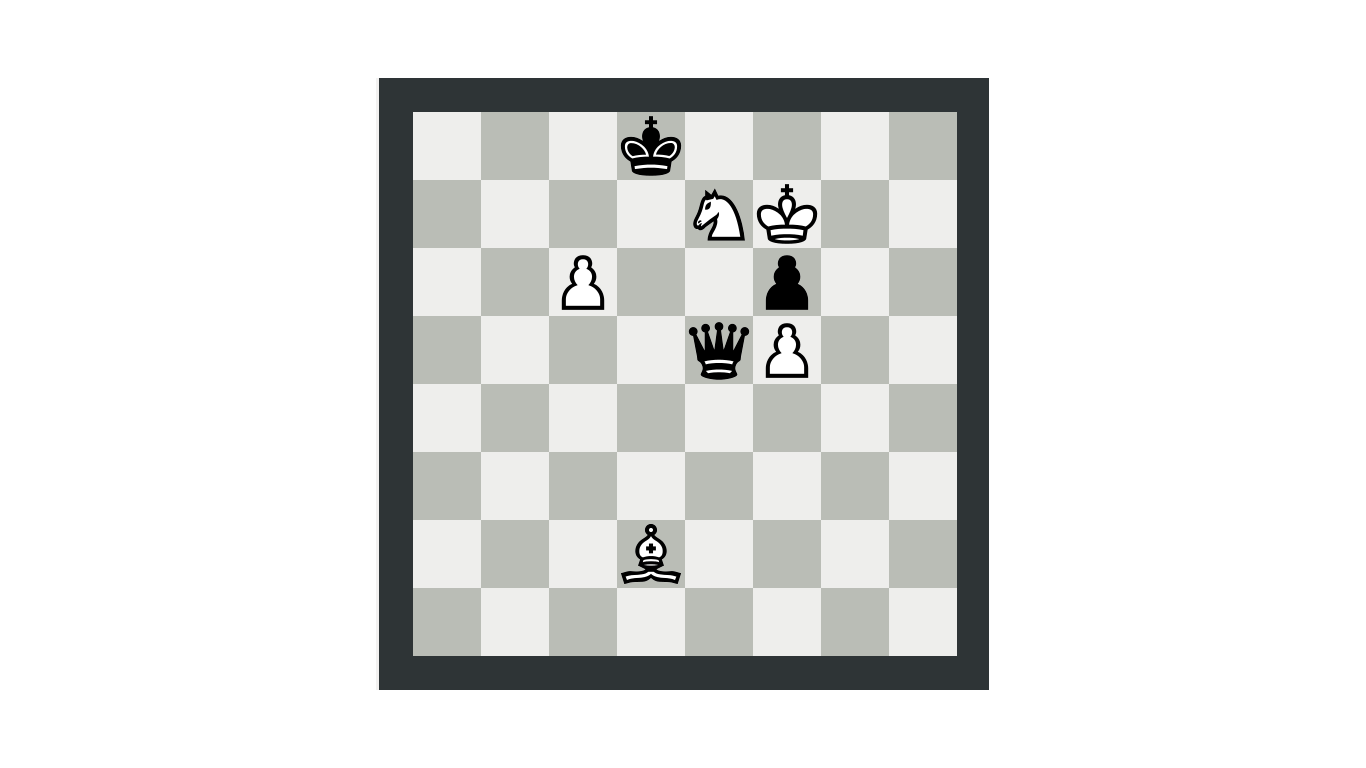
\includegraphics[scale=0.2]{partida2.png}
%\caption{Reto ajedrecístico}\label{partida}
%\end{figure}

\end{multicols}
%\noindent
\vspace{0.5cm}
\centering
\includegraphics[scale=0.3]{aihbbgje.jpg}

\newpage


%%% Local Variables:
%%% mode: latex
%%% TeX-master: "jugando"
%%% End:
